\documentclass[10pt] {article}
\usepackage[portuguese]{babel}
\usepackage[utf8]{inputenc}
\usepackage{graphicx}
\usepackage[labelformat=empty]{caption}
\usepackage{tikz}
\setcounter{secnumdepth}{5}
\setcounter{tocdepth}{5}

\usepackage{geometry} % Required to change the page size to A4
\geometry{a4paper} % Set the page size to be A4 as opposed to the default US Letter

\usepackage{tikz}
\usepackage{pgfplots}

\usepackage{indentfirst} %Identação nos parágrafos iniciais

% Code
\usepackage{listings}
\lstset{language=Java, breaklines=true, basicstyle=\footnotesize} % Especificar Haskell, mudar de linha quando acabar espaço, diminuir tamanho da letra.
\usepackage{fixltx2e} % Corrige alguns erros
\begin{document}

\title{Relatório Trabalho Prático Java \\ $\small{Grupo 13}$}

\maketitle

%--------------------------------
% Group Members
%--------------------------------
\begin{figure}[!htb]
\minipage{0.31\textwidth}
  
\includegraphics[width=\linewidth]{jc.jpg}
  \caption{João Costa A70563}\label{fig:awesome_image1}
\endminipage\hfill
\minipage{0.29\textwidth}
  
\includegraphics[width=\linewidth]{ls.jpg}
  \caption{Leandro Salgado A70949}\label{fig:awesome_image2}
\endminipage\hfill
\minipage{0.32\textwidth}%
  
\includegraphics[width=\linewidth]{ma.jpg}
  \caption{Martinho Aragão A72205}
\endminipage
\end{figure}

\newpage

\tableofcontents

\newpage

\section{Introdução}

Este relatório aborda a resolução do projeto prático em Java de LI3.
O Projeto, denominado Gesthiper, baseia-se num programa de gestão de hipermercados o qual depende de uma lista de clientes, uma lista de produtos e uma lista de compras efetuadas.

Cada uma destas listas deve estar num ficheiro .txt e para cada um dos ficheiros o programa percorre o ficheiro, executando operações que permitam guardar estes dados em memória.
Para ajudar nesta tarefa repartiu-se as tarefas em quatro módulos módulos.
Estes módulos são: um catálogo de clientes; um catálogo de produtos; um módulo de contabilidade; um módulo de compras.

De forma a preservar o encapsulamento de dados disponibilizou-se uma API de
forma a que o utilizador apenas possa aceder através destas funções públicas.

Depois dos ficheiros serem carregados o utilizador é capaz de executar uma lista de querys que foi fornecida pela equipa docente.
Para responder às diferentes queries utiliza-se as funções definidas nas API dos diferentes módulos já referidos bem como código auxiliar presente no \emph{main}, programa principal.

Ao longo deste relatório aborda-se assim as decisões tomadas na implementação do projeto, nomeadamente quais as estruturas utilizadas para criar cada um dos módulos e as suas APIs.


\newpage
\section{Classes}
Na seguinte secção vamos explicar as classes que decidimos criar para a resolução do projeto, incluindo diagramas e explicação das estruturas escolhidas para cada classe.

% ClientsCatalog
\subsection{ClientsCatalog}

Para guardar os clientes presentes no ficheiro de clientes, criámos a classe \textbf{ClientsCatalog} que irá guardar clientes e manter a lista dos que não realizaram nenhuma compra.

Para além disso cria a lista com todos os códigos de cliente a partir de uma letra inicial do código.

Fica aqui o código que define as variáveis de instância:

\begin{lstlisting}
public class ClientsCatalog {
	/* Codigo de cliente -> Cliente */
	private TreeSet<String> clients;
	/* Lista de clientes que nao compraram nenhum produto */
	private TreeSet<String> unused_clients;
}
\end{lstlisting}


Uma das vantagens desta implementação é que, quando o utilizador decide ler um novo ficheiro de compras, não é necessário percorrer a lista de todos os clientes e voltar a inserir na lista de clientes que nunca compraram nada para depois retirar à medida que aparecem no ficheiro de compras.
Como \textbf{String} são imutáveis basta correr o código:
$unused\_clients = clients.clone();$ e a variável $unused\_clients$ passa agora a ter novamente a lista de todos os clientes que estão no catálogo de clientes.

%ProductsCatalog
\subsection{ProductsCatalog}

A classe \textbf{ProductsCatalog} é responsável por guardar todos os códigos de produtos existentes no ficheiro de produtos assim como guardar a lista de produtos que ninguém comprou.

Para guardar as duas listas referidas usamos a classe \textbf{TreeSet} pois como os códigos de produtos são apenas do tipo \textbf{String} a pesquisa num \textbf{TreeSet} é rápida.

A declaração das variáveis de instância segue de seguinte:

\begin{lstlisting}
public class ProductsCatalog {
	/* Lista de todos os codigos de produto */
	private TreeSet<String> products;
	/* Lista de produtos que ninguem comprou */
	private TreeSet<String> unused_products;
}
\end{lstlisting}


Tal como no caso da classe \textbf{ClientsCatalog} sempre que for necessário voltar a ler o ficheiro de compras basta reconstruir a lista de todos os códigos de produto na lista dos produtos que ninguém comprou, correndo:
$unused\_products = products.clone();$.

\newpage
\subsection{Sale}

Para o módulo de Compras é necessário guardar informação sobre todas as compras válidas quem as fez, quando, o que comprou, quantos unidades comprou, o tipo da compra e o total pago.

A classe \textbf{Sale} trata de guardar informação relativa a uma compra, guardando o código do produto comprado, as unidades, o tipo da compra (promocional ou normal) e o total gasto.

Fica em seguida a declaração das variáveis de instância:

\begin{lstlisting}
public class Sale {
	/* Codigo do produto */
	private String product;
	/* Numero de unidades compradas */
	private int units;
	/* Total gasto na compra */
	private float price;
	/* Tipo da compra */
	private boolean type;
}
\end{lstlisting}


Foi usado um valor do tipo \textbf{boolean} para guardar o tipo de compra pois apenas há duas opções, ou é uma compra normal, à qual associamos o valor $false$, ou é uma compra promocional, à qual associamos o valor $true$.

\subsection{ProductTotalSales}

Para o módulo de Contabilidade é necessário guardar informação sobre o total de vendas de um produto ou seja, faturação e unidades divididos entre promoção e vendas normais.

Assim a classe \textbf{Contabilidade} trata de guardar informação relativa a cada um destes dados, ao multiplicar as unidades e preço por unidade de uma venda.

De seguida declara-se as variáveis de instância:

\begin{lstlisting}
public class Sale {
  private String product;         /* Codigo de Produto */
  private int normalUnits;        /* Quantas unidades vendidas ao preco normal */
  private int promoUnits;         /* Quantas unidades vendidas ao preco de promocao */
  private double normalRevenue;   /* Faturacao total a preco normal */
  private double promoRevenue;    /* Faturacao total a preco de promocao */

}
\end{lstlisting}

\subsection{Classes Auxiliares}
\subsubsection{ParSaleClient}

A classe \textbf{ParSaleClient} foi criada para responder à necessidade de queries que necessitavam de obter informação relativa ao número total de vendas assim como o número total de clientes diferentes que tinham efectuado essas compras.

Para guardar esta informação usou-se então apenas duas variáveis de instância aqui declaradas:

\begin{lstlisting}
public class ParSaleClient {
	/* Numero total de vendas */
	private int num_sales;
	/* Numero total de diferentes clientes que efectuaram compras */
	private int num_clients;
}
\end{lstlisting}

\subsubsection{ParClientFat}

Para resolver a query 5 é necessário guardar informações relativas ao número de clientes que compraram um produto e total faturado desse produto por mês. Para isso definimos a classe \textbf{ParClientFat} cuja definição das variáveis de
instância é a seguinte:

\begin{lstlisting}
public class ParClientFat {
	/* Produto a qual esta associado */
	private String product;
	/* Lista de clientes que compraram o produto */
	private Set<String> clients;
	/* Total faturado */
	private float invoiced;
}
\end{lstlisting}


Obviamente não era preciso guardar a informação sobre a qual produto está relacionado visto que o produto é definido pelo utilizador e não muda durante a execução da query.

A lista de clientes foi implementada usando um \textbf{Set} pois garante a ausência de elementos repetidos.

Relativamente à 5 é criado um \textbf{ArrayList} com 12 entradas, um para cada mês, e cada um contêm uma instância de \textbf{ParClientFat} relativa a esse mês.

\subsubsection{TripNumProdFat}

Para poder guardar informação relativa ao número de compras, número de diferentes produtos comprados e total faturado por mês para um dado cliente houve necessidade de criar uma nova classe que guardasse estas informações-

A definição das variáveis de instância é a seguinte:

\begin{lstlisting}
public class TripNumProdFat {
	/* Numero total de vendas */
	private int num_sales;
	/* Lista de produtos que comprados */
	private Set<String> products;
	/* Total faturado */
	private float total;
}
\end{lstlisting}


Foi necessário utilizar um Set para guardar os códigos de produtos pois era necessário garantir que o mesmo produto não era contabilizado várias vezes.
Utilizou-se um \textbf{TreeSet} pois a pesquisa é rápida e garante que não existem elementos repetidos.

A figura ~\ref{fig:catprodutos} na página ~\pageref{fig:catprodutos} é um exemplo de um TreeSet de códigos de produtos.

\subsubsection{TripProdCliUnits}

Para a execução da query 8 é necessário guardar informações relativas ao número unidades vendidas de um produto
bem como o número de diferentes clientes que compraram esse produto.

A declaração das variáveis de instância é a seguinte:

\begin{lstlisting}
public class TripProdCliUnits {
	/* Produto associado */
	private String product;
	/* Lista de clientes que compraram o produto */
	private TreeSet<String> clients;
	/* Total de unidades vendidas */
	private int units;
	...
}
\end{lstlisting}


Obviamente não era preciso guardar a informação sobre a qual produto está relacionado visto que o produto é definido pelo utilizador e não muda durante a execução da query.

A lista de clientes foi implementada usando um \textbf{Set} pois garante a ausência de elementos repetidos.

Relativamente à 5 é criado um \textbf{ArrayList} com 12 entradas, um para cada mês, e cada um contêm uma
instância de \textbf{ParClientFat} relativa a esse mês.

\subsubsection{ParClientQuant}

A resolução das queries 9 e 10 requeriam que a cada código de cliente estivesse associado um número de unidades e, no caso da query 10, um total faturado por esse cliente. Assim, foi definida a classe \textbf{ParClientQuant} cuja
definição das variáveis de instância é a seguinte:

\begin{lstlisting}
public class ParClientQuant {
    /* client code */
	private String client_code;
	/* number of products the client bought */
    private int num_products;
    /* how much the client spent with the products */
    private double fat;
}
\end{lstlisting}


Na  9, é apenas necessário associar a um código de cliente, o número de produtos diferentes que esse cliente comprou.
Como tal, a variável \textbf{fat} é apenas utilizada na query 10, onde é necessário associar a um código de cliente, não só o número de unidades de um produto que o cliente comprou, como o total gasto pelo cliente relativo a esse produto.

\subsubsection{ParProductUnits}

De modo a resolver a query 7 foi necessário desenvolver uma classe que associasse um valor a um código de produto.
Desta forma, a classe \textbf{ParProductUnits} foi definida. A definição das suas variáveis de instância é a seguinte:

\begin{lstlisting}
public class ParProductUnits {
	/* product code */
    private String product_code;
    /* number of times the product was bought */
    private int num_sold;
\end{lstlisting}


Esta classe associa o número de vezes que um produto foi comprado ao código do dito produto.
Assim, pudemos evitar a utilização de estruturas de dados demasiado complexas que conseguissem associar um \textbf{int} a uma \textbf{String}.

\newpage
\section{Módulos}
\subsection{Catálogo de Clientes}

Para manter uma cópia de todos os clientes que existem para, por exemplo, verificar se uma compra é válida, é necessário
criar um catálogo de clientes.
Visto que o catálogo apenas deveria guardar os códigos de clientes decidimos criar a classe \textbf{ClientsCatalog} que guarda todos os códigos de cliente do tipo \textbf{String} num TreeSet proporcionando assim uma pesquisa rápida.

\begin{figure}[ht!]
\centering
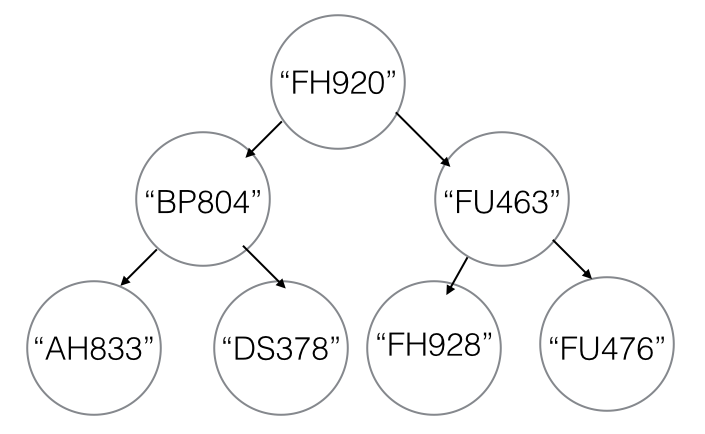
\includegraphics[width=90mm]{catclientes.png}
\caption{Exemplo de um TreeSet de clientes}
\end{figure}

\newpage
\subsection{Catálogo de Produtos}

O catálogo de clientes foi implementado usando a class  \textbf{ProductsCatalog} que basicamente guarda os códigos dos produtos num TreeSet.
Como os códigos dos produtos são apenas \textbf{String} a árvore fica então ordenada alfabeticamente e a procura é rápida.

\begin{figure}[ht!]
\centering
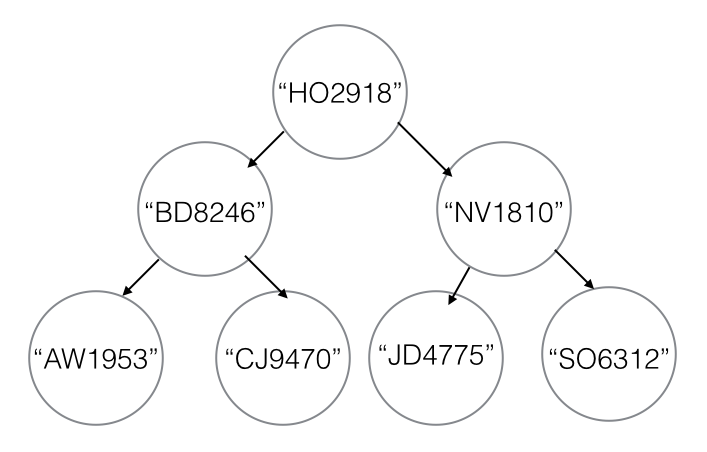
\includegraphics[width=90mm]{catprodutos.png}
\caption{Exemplo de um TreeSet de produtos}
\label{fig:catprodutos}
\end{figure}

\subsection{Compras}

O módulo de compras é responsável por guardar todas as compras válidas, relacionando quais os clientes que fizeram essas compras e quando.
Desta forma é possivel consultar as vendas por mês se assim for desejado.

Como então era necessário conseguir dividir as compras por mês utilizou-se um \textbf{ArrayList} com 12 entradas, e em cada uma destas entradas existe um \textbf{TreeMap\textless String, ArrayList\textless Sale\textgreater\textgreater} que mapeia um código de cliente para a lista de compras efectuadas por esse cliente.
Usando um \textbf{TreeMap} permite uma procura rápida por um dado cliente e o arraylist permite um acesso directo às compras de um determinado mês.

A declaração das variáveis de instância é a seguinte:

\begin{lstlisting}
public class Sales {
	ArrayList<TreeMap<String, ArrayList<Sale>>> sales;

	...
}
\end{lstlisting}

Para mais facilmente entender a implementação incluimos uma figura da estrutura:

\begin{figure}[ht!]
\centering
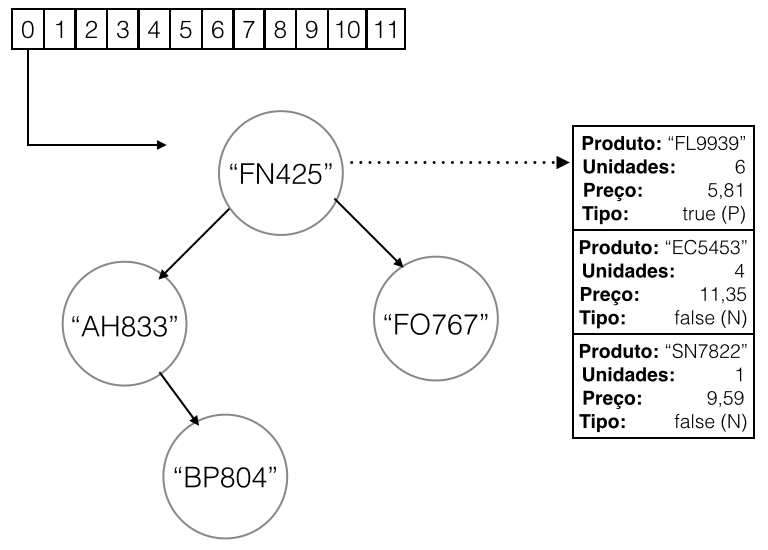
\includegraphics[width=90mm]{sales.png}
\caption{Exemplo da estrutura com as compras de Janeiro do cliente "FN425"}
\label{fig:sales}
\end{figure}

\subsection{Contabilidade}

O módulo de contabilidade é responsável por guardar a faturação mensal de cada um dos produtos.
Desta forma pretende-se que seja possível obter facilmente a faturação total de um mês, analisar as vendas de um produto mensalmente, e as suas vendas todais num ano.

Como então era necessário conseguir dividir as vendas por mês utilizou-se um \textbf{ArrayList} com 12 entradas, e em cada uma destas entradas existe um \textbf{TreeMap\textless String, ProductTotalSales\textgreater} que mapeia um código de produto para a informação de faturação total do mesmo.
Usando um \textbf{TreeMap} permite uma procura rápida por um dado produto e o arraylist permite um acesso directo às vendas de um determinado mês.

A declaração das variáveis de instância é a seguinte:

\begin{lstlisting}
public class Accounting {
/* Informacao de faturacao por mes e por produto */
  private ArrayList<TreeMap <String,ProductTotalSales>> accounting;

  ...
}

\end{lstlisting}

Para mais facilmente entender a implementação incluimos uma figura da estrutura:

\begin{figure}[ht!]
\centering
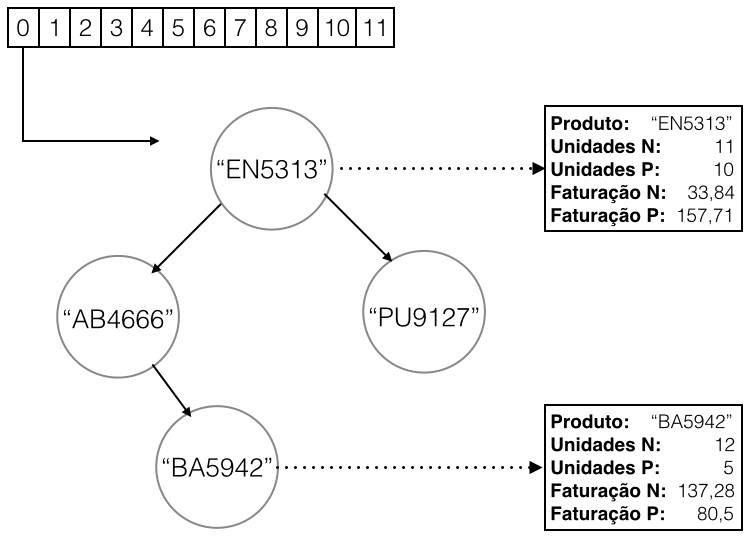
\includegraphics[width=90mm]{accounting.jpg}
\caption{Exemplo da estrutura com algumas vendas de Janeiro descritas}
\label{fig:sales}
\end{figure}

% UI
\newpage
\section{Interface Utilizador}

Para ser possível realizar as queries foi necessário criar um menu inicial que não é mais que uma lista com opções numeradas e cada opção tem a sua descrição, a partir deste menu inicial o utilizador apenas tem que introduzir o número da opção que deseja aceder.

Para algumas das queries listas de \emph{Strings} têm de ser apresentadas, essas listas podem variar muito  em tamanho e então era necessário uma maneira de as apresentar no ecrã, sem sacrificar a leitura das mesmas.

Para isso foi criado um método \emph{paginate} que recebendo um array de strings apresenta ao utilizador a possibilidade de navegar nas páginas, especificando se quer ir para a próxima página, para a página anterior, para uma página especifica ou então voltar ao menu inicial.

Também há queries que requerem a apresentação de tabelas, para cada uma dessas queries foi utilizado \emph{String.format} que trata de formatar a palavra para apresentar numa tabela ao terminal do utilizador.
\newpage
\section{Diagrama de Classes}
\par De seguida é apresentado o Diagrama de classes gerado no BlueJ com os ficheiros .java usados para a entrega, é
necessário ter atenção que o BlueJ por algum motivo não cria todas as ligações, por exemplo, através das declarações das
variáveis de instância da classe \color{blue} \textbf{Hypermarket} \color{black}:

\begin{lstlisting}
public class Hypermarket {
	private ProductsCatalog p_cat;
   	private ClientsCatalog  c_cat;
    	private Sales sales;
    	private Accounting accounting;
	...
}
\end{lstlisting}

\par podemos ver que ele depende das classes: \color{blue} \textbf{ProductsCatalog, ClientsCatalog, Sales} \color{black} e
\color{blue} \textbf{Accounting} \color{black}, contudo o BlueJ não cria ligação a todas estas classes, não conseguimos
descobrir qual era o problema que causava este comportamento.

\begin{figure}[ht!]
\centering
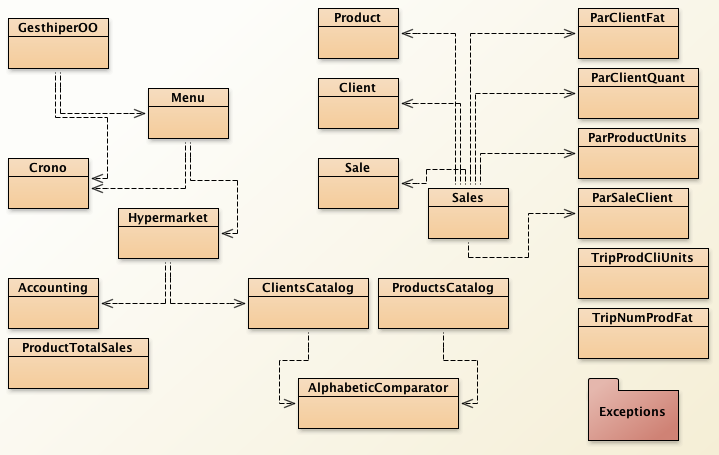
\includegraphics[width=150mm]{diagram.png}
\caption{Diagrama de classes}
\label{fig:sales}
\end{figure}

\newpage
\section{Gráficos e Resultados}

\par Para verificar qual a melhor classe a usar para fazer a leitura dos ficheiros corremos testes para as classes
\textbf{BufferedReader} e para a classe \textbf{Scanner}, realizando testes fazendo parsing da string e criando instância
da class \textbf{Sale} e testes sem parsing.
\par De seguida ficam tabelas com os resultados obtidos e também um gráfico para comparação de resultados.

\begin{table}[h]
\centering
\caption{Resultados Sem Parsing}
\label{my-label}
\begin{tabular}{l|l|l|ll}
\cline{2-3}
                                   & BufferedReader (Sem Parsing) & Scanner (Sem Parsing) &  &  \\ \cline{1-3}
\multicolumn{1}{|l|}{500k Compras} & 0,127064 seg                 & 2,015564 seg          &  &  \\ \cline{1-3}
\multicolumn{1}{|l|}{1M Compras}   & 0,155963 seg                 & 3,479728 seg          &  &  \\ \cline{1-3}
\multicolumn{1}{|l|}{3M Compras}   & 0,478711 seg                 & 10,409572 seg         &  &  \\ \cline{1-3}
\end{tabular}
\end{table}

\begin{table}[h]
\centering
\caption{Resultados Parsing}
\label{my-label}
\begin{tabular}{l|l|l|ll}
\cline{2-3}
                                   & BufferedReader (Parsing) & Scanner (Parsing) &  &  \\ \cline{1-3}
\multicolumn{1}{|l|}{500k Compras} & 0,340476 seg             & 0,927688 seg      &  &  \\ \cline{1-3}
\multicolumn{1}{|l|}{1M Compras}   & 0,586160 seg             & 1,690759 seg      &  &  \\ \cline{1-3}
\multicolumn{1}{|l|}{3M Compras}   & 1,478137 seg             & 4,963618 seg      &  &  \\ \cline{1-3}
\end{tabular}
\end{table}

\begin{figure}[ht!]
\centering
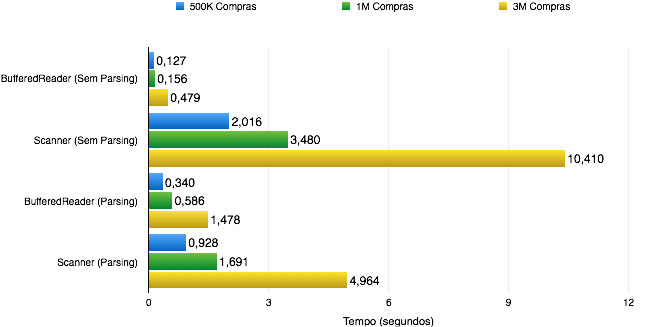
\includegraphics[width=150mm]{filegraph.png}
\caption{Resultados dos testes de leitura de ficheiros}
\label{fig:sales}
\end{figure}

\newpage

Assim pode-se concluir que apesar de  \color{blue}\textbf{BufferedReader}\color{black} ser mais rápido em todas as situações, ao contrário do que era esperado por nos a class  \color{blue}\textbf{Scanner}\color{black} tem um comportamento mais eficiente durante parsing, pois é esta a sua principal utilização.

\par Também foram realizados testes para outras estruturas de dados para ver a diferença de tempo de execução para as
queries 8, 9 e 10. Foram consideradas 4 situações diferentes, a primeira situação é onde a estrutura do módulo de
compras, a class \color{blue} \textbf{Sales} \color{black} tem a sua estrutura definida da seguinte forma:

\begin{lstlisting}
public class Sales {
	ArrayList<TreeMap<String, ArrayList<Sale>>> sales;
	...
}
\end{lstlisting}

\par Na segunda situação a estrutura foi modifica para em vez de utilizar \color{blue} \textbf{TreeMap} \color{black} utilizar um
\color{blue} \textbf{HashMap} \color{black} . Ficando então a estrutura definida da seguinte forma:

\begin{lstlisting}
public class Sales {
	ArrayList<HashMap<String, ArrayList<Sale>>> sales;
	...
}
\end{lstlisting}

\par Na terceira situação a estrutura foi modifica para em vez de utilizar \color{blue} \textbf{ArrayList} \color{black} utilizar a
classe  \color{blue} \textbf{Vector} \color{black} . Ficando então a estrutura definida da seguinte forma:

\begin{lstlisting}
public class Sales {
	Vector<TreeMap<String, Vector<Sale>>> sales;
	...
}
\end{lstlisting}

\par A útima situação, situação 4 é a mistura da situação 2 e 3, ficando a estrutura definida da seguinte forma:

\begin{lstlisting}
public class Sales {
	Vector<HashMap<String, Vector<Sale>>> sales;
	...
}
\end{lstlisting}

\par Para medir os tempos executamos as queries 8, 9 e 10. Na query 8 utilizamos 1000 produtos como o número base
para os testes e na query 9 utilizamos 1000 clientes. Para a query 10, para cada uma das situações corremos 5 vezes,
para os produtos: "HO2915", "GF7879", "EN3727", "TM3887", "KN1847" e 1000 clientes, no final calculamos a média destas 5
execuções e foi o tempo que registamos.
\par De seguida apresentamos a tabela dos tempos registados seguido de um gráfico que irá ajudar na conclusão destes
testes de performance das diferentes estruturas.

\newpage

\begin{table}[h]
\centering
\caption{Resultados dos Testes às Estruturas}
\begin{tabular}{l|l|l|l|l|}
\cline{2-5}
                               & Situação 1 & Situação 2 & Situação 3 & Situação 4 \\ \hline
\multicolumn{1}{|l|}{Query 8}  & 2,600 seg  & 0,576 seg  & 2,737 seg  & 0,614 seg  \\ \hline
\multicolumn{1}{|l|}{Query 9}  & 0,451 seg  & 0,347 seg  & 0,470 seg  & 0,314 seg  \\ \hline
\multicolumn{1}{|l|}{Query 10} & 0,070 seg  & 0,077 seg  & 0,071 seg  & 0,082 seg  \\ \hline
\end{tabular}
\end{table}

\begin{figure}[ht!]
\centering
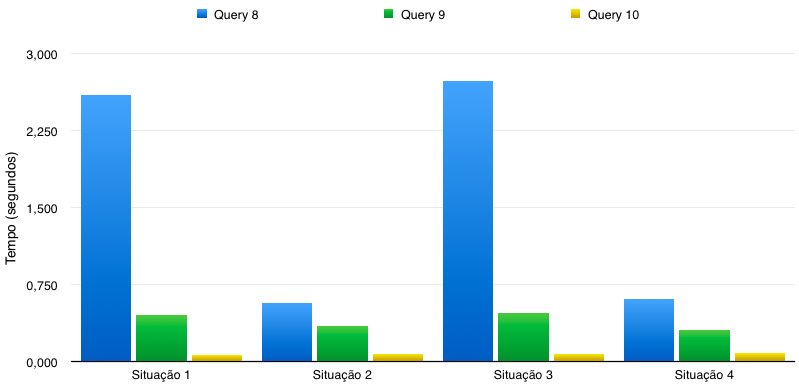
\includegraphics[width=150mm]{graphstruct.png}
\caption{Resultados dos testes das diferentes estruturas}
\label{fig:sales}
\end{figure}

\par Entre as 4 situações, nota-se claramente uma disparidade enorme nos resultados da query 8 para a situação 1 e 3.
Ou seja, comparando \color{blue} \textbf{HashMap} \color{black} com \color{blue} \textbf{TreeMap} \color{black} é evidente que
o 1.º apresenta um comportamento muito mais eficiente nas necessidades da query 8.
De facto, as outras situações e queries não divergem substancialmente.

\par Demonstra-se assim que se deveria ter implementado um \color{blue} \textbf{HashMap} \color{black} na estrutura da classe \color{blue}\textbf{Sales}\color{black}.

\newpage

\section{Conclusão}

A implementação de um programa de gestão de hipermercados em Java provou ser mais fácil quando comparado á implementação em C.
Tal deve-se, em grande maioria, à necessidade de definir de raiz um grande número de funções como por exemplo estruturas.
Esta vantagem de implementação permite desenvolver soluções adicionais que teriam um custo considerável em C.

Assim sendo foi possível concretizar as várias queries com maior facilidade, sem prejudicar a sua velocidade, graças à facilidade em trocar e testar diferentes estruturas, desde que estas partilhem da mesma API.

Em jeito de esclarecimento, o trabalho foi realizado em inglês por uma questão de aprendizagem no que toca à utilização de ferramentas de código aberto, neste caso git através do GitHub.
\end{document}
